% Chapter 1

\chapter{Resultados} % Main chapter title

\label{Cap_Res} % For referencing the chapter elsewhere, use \ref{Chapter1} 

En las tareas contempladas en cada uno de los experimentos realizados (i.e tarea de detección binaria y la escala de confianza), se encontró evidencia de los patrones de respuesta identificados como parte del Efecto Espejo en al menos tres cuartas partes de los participantes. En el Experimento 1, diecisiete de los veinte participantes mostraron el patrón de respuesta esperado en la tarea de detección visual y dieciocho en la escala de confianza. A su vez, en el Experimento 2 los patrones asociados con el Efecto Espejo aparecieron en diecinueve de los veintiun participantes, en ambas tareas. De acuerdo a una prueba binomial, todas estas proporciones son estadísticamente significativas contra el azar (p=0.0025 y p=0.0004 para las proporciones reportadas en el Experimento 1, respectivamente; p=0.0002 para el Experimento 2).\\

El análisis de datos está organizado en torno a los siguientes puntos:

\begin{itemize}
\item \textbf{Verificar que las condiciones de dificultad son de hecho diferentes.}
Dado que las condiciones de dificultad fueron diseñadas en función a lo reportado en la literatura, es preciso corroborar que las manipulaciones implementadas en el diseño de las figuras de Ebbinghaus tuvieron un efecto en el desempeño de los participantes. De acuerdo con la TDS, el parámetro d' que cuantifica la discriminabilidad entre señales y ruido a partir de la distancia entre la media de las distribuciones correspondientes, obtenido en cada condición sería nuestro mejor estimador para responder a esta cuestión. En concreto, se espera que:
\begin{center}
 D'(2 o 3 círculos externos) $>$ D'(7 u 8 círculos externos)\\
 \end{center}

 \item \textbf{Comparar las tasas de Hits y Falsas Alarmas entre condiciones.}
Evaluar si, tal y como se reporta en la literatura en memoria de reconocimiento, las diferencias en la ejecución de los participantes entre dos condiciones de dificultad se presentan 'en dos sentidos': en la condición identificada como 'fácil' por tener una mayor discriminabilidad, se cometen tanto más aciertos como menos errores, relativo a una segunda condición con menos discriminabilidad. De acuerdo con la literatura en Memoria de Reconocimiento que aborda el Efecto Espejo, se tomaría como evidencia del mismo los siguientes patrones entre los Hits y Falsas Alarmas cometidos en cada condición:
\begin{center}
Hits(A) $>$ Hits(B)\\
Falsas Alarmas(B) $>$ Falsas Alarmas(A)\\
\end{center}

\item \textbf{Comparar el puntaje de confianza promedio asignado a cada tipo de ensayo entre las condiciones.}
De acuerdo con 
\begin{center}
Confianza(A) $>$ Confianza(B)\\
De acuerdo con la conversión establecida para las respuestas emitidas ('1','2', y '3') y la escala de confianza, esto debería traducirse en:\\
Puntaje(AS) $>$ Puntaje(BS)\\
Puntaje(AN) $<$ Puntaje(BN)\\
\end{center}

\item \textbf{Réplica de controles reportados en la literatura.}
	\begin{itemize}
	\item Descartar relación entre el tipo de estímulo y los tiempos de respuesta.
	\item Comprobar la extensividad de las diferencias encontradas en la tarea con la escala.
	\end{itemize}
\end{itemize}

Cada uno de estos puntos será desarrollado en detalle desde dos enfoques estadísticos distintos:\\

\begin{itemize}
\item La réplica de lo reportado en la literatura.\\

Considerando que el objetivo principal de la investigación aquí desarrollada fue probar la generabilidad de los patrones de respuesta identificados como Efecto Espejo dentro del estudio de la Memoria de Reconocimiento, se

\item El desarrollo de modelos Bayesianos para la estimación paramétrica y la evaluación de efectos.\\



\end{itemize}

\section{Las condiciones de dificultad son diferentes}

Las condiciones de dificultad propuestas para los experimentos realizados, se construyeron con base en los hallazgos reportados por \parencite{Masaro1971} en cuanto al efecto que tienen las diversas variables que componen las figuras de Ebbinghaus. De acuerdo con estos autores, una de las variables cuyo impacto en la intensidad de la ilusión de Ebbinghaus es más claro, es el número de círculos que aparecen en torno al círculo central.



\begin{figure}[th]
\centering
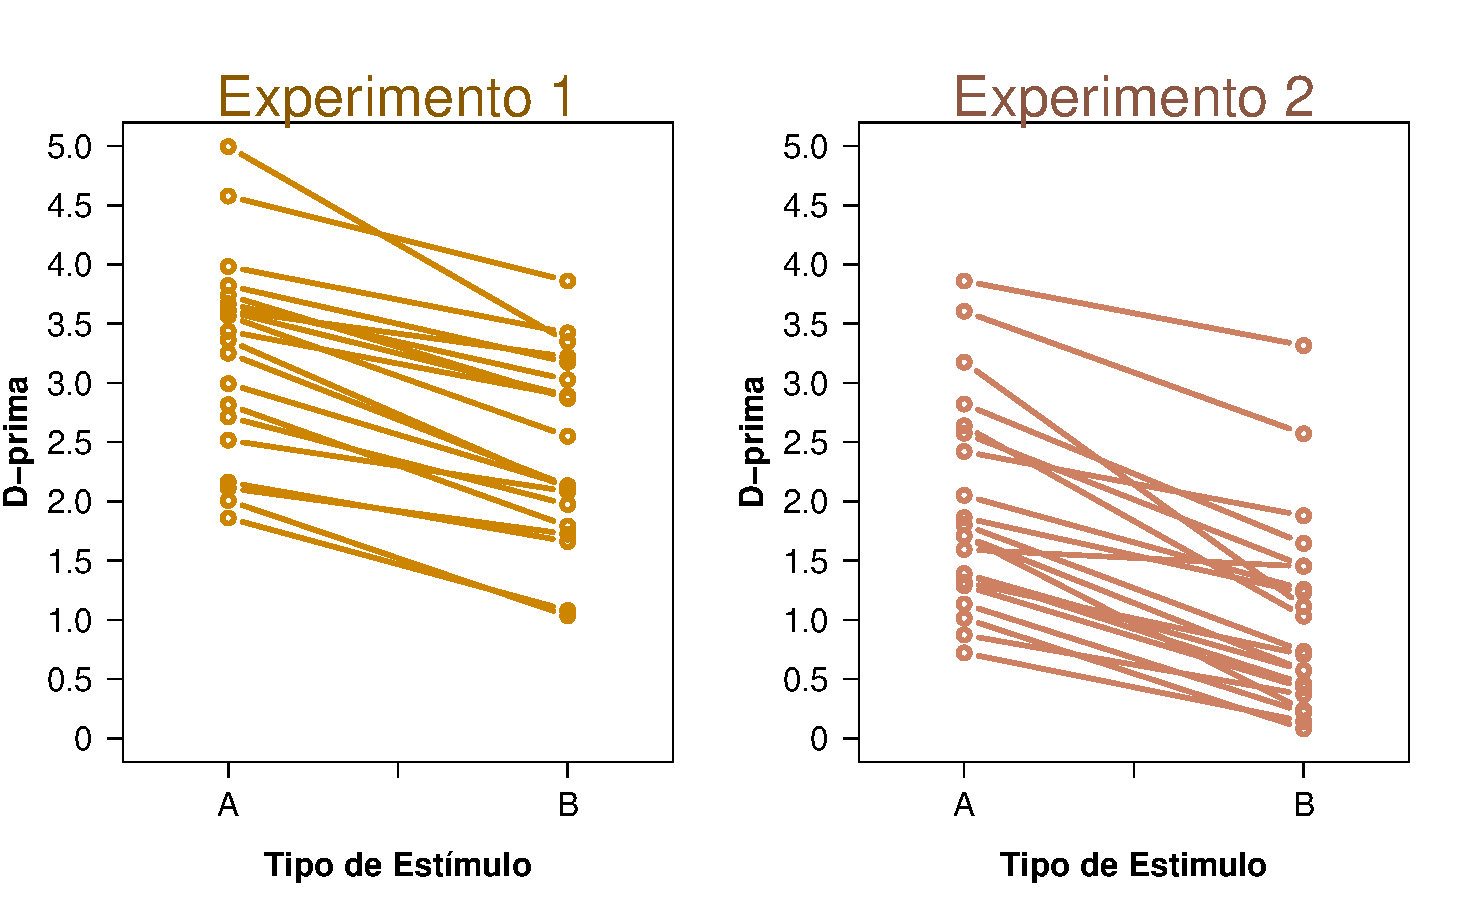
\includegraphics[width=0.80\textwidth]{Figures/Diff_D_E1yE2}
%\decoRule
\caption[Diferencias en Discriminabilidad (Comprobando diferencias entre condiciones)]{ }
\label{fig:Diff_D}
\end{figure}

\subsection{Análisis 1: Prueba T para comparar las medias de d' por cada condición}

\begin{table}
\caption[Prueba T]{Diferencias en d'}
\label{Tabla_t-HitsyFA}
\centering
\begin{tabular}{l | c c c c}
\toprule
%\tabhead{Groups} & \tabhead{Treatment X} & \tabhead{Treatment Y} \\
\textbf{T-test} & \textbf{$\mu$ A} & \textbf{$\mu$ B} & \textbf{T}  & \textbf{P value}\\
\midrule
Experiment 1 & 3.240 & 2.448 & -3.0587 & 0.0020 \\
Experiment 2 & 1.950 & 1.022 & -3.4972 & 0.0005 \\
\bottomrule
\end{tabular}
\end{table}


\subsection{Análisis 2: Modelo jerárquico bayesiano: Modelo Delta para diferencias en d'}

\begin{figure}[th]
\centering
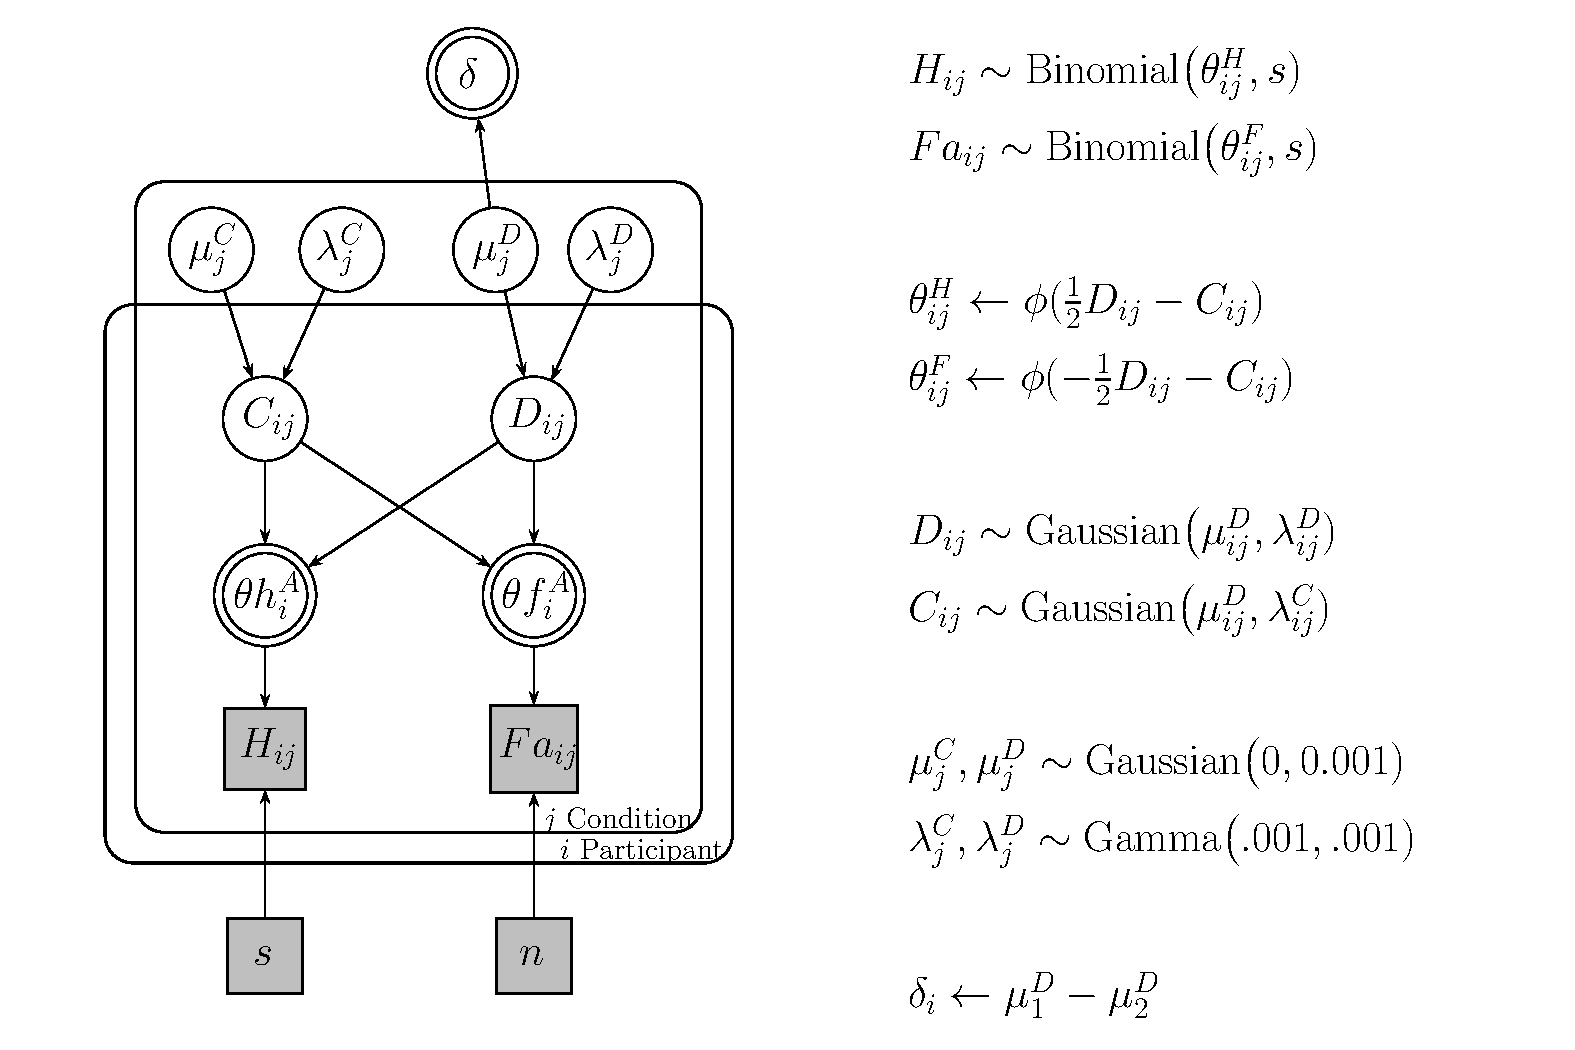
\includegraphics[width=0.80\textwidth]{Figures/Model_Delta_Diff_D}
%\decoRule
\caption[Diferencias en Tasas (Comprobando diferencias entre condiciones)]{Comparación intrasujeto de}
\label{fig:Mod_Delta}
\end{figure}


%----------------------------------------------------------------------------------------

\section{Diferencias en las Tasas de Hits y Falsas Alarmas}

\begin{figure}[th]
\centering
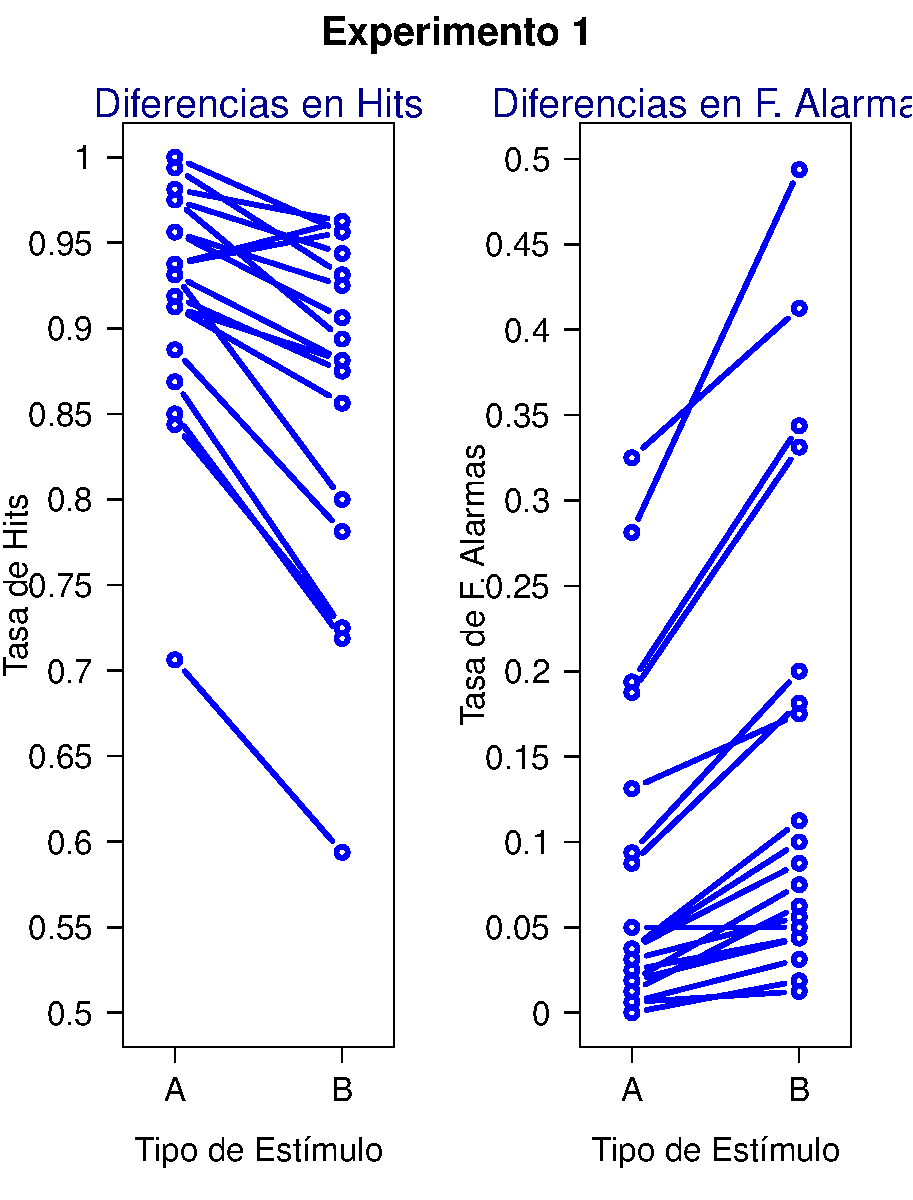
\includegraphics[width=0.80\textwidth]{Figures/Diff_Rate_E1}\\ 
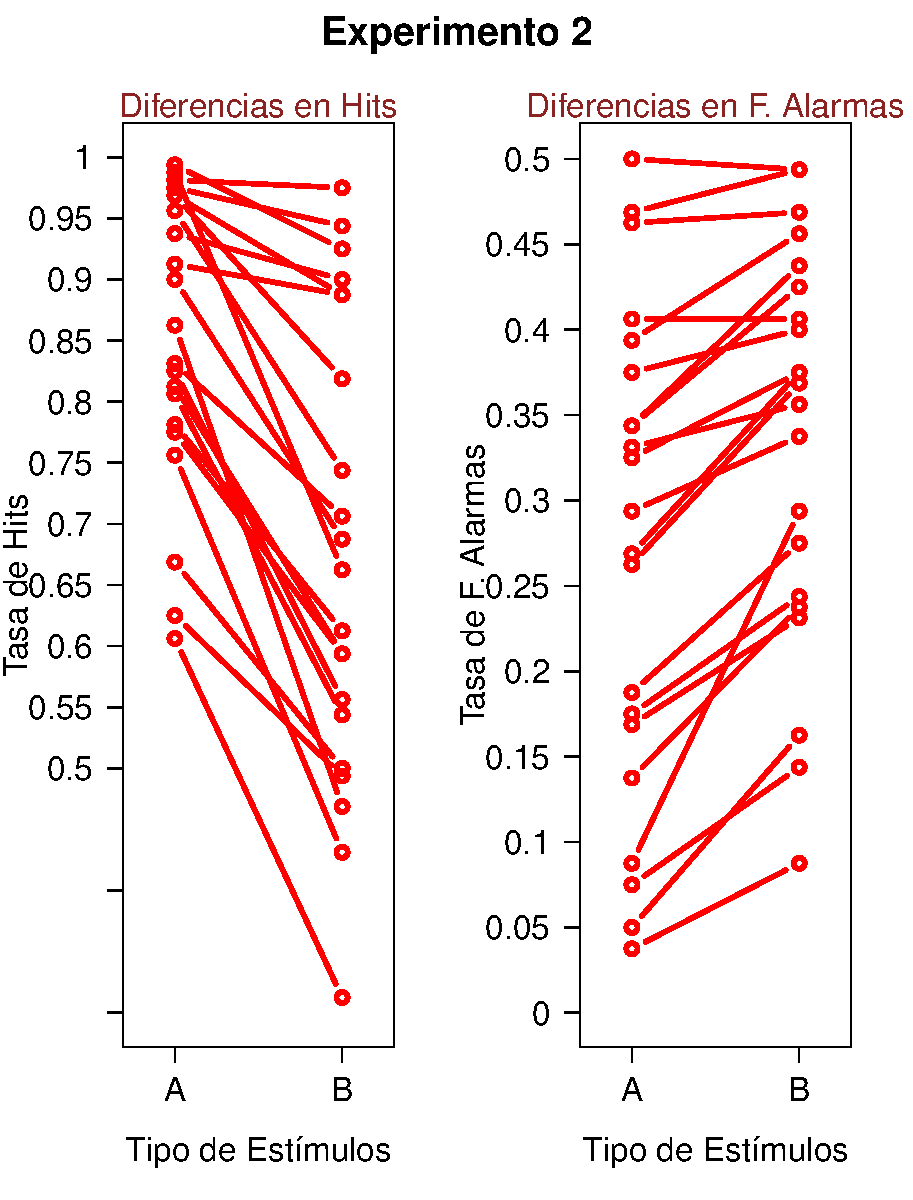
\includegraphics[width=0.80\textwidth]{Figures/Diff_Rate_E2}
%\decoRule
\caption[Diferencias en Tasas (Comprobando diferencias entre condiciones)]{Comparación intrasujeto de}
\label{fig:Diff_Rate}
\end{figure}


\subsection{Análisis 1: Prueba T}



\begin{table}
\caption[Prueba T]{Diferencias en Hits y Falsas Alarmas entre los tipos de estímulos (Experimento 1 y 2)}
\label{Tabla_t-HitsyFA}
\centering
\begin{tabular}{l l | c c c c}
\toprule
%\tabhead{Groups} & \tabhead{Treatment X} & \tabhead{Treatment Y} \\
\textbf{T-test} & \textbf{} & \textbf{$\mu$ A} & \textbf{$\mu$ B} & \textbf{T} & \textbf{P value}\\
\midrule
Exp 1 & Hits & 0.922 & 0.860 & -2.4348 & 0.0098 \\
Exp 1 & FA & 0.08 & 0.143 & 1.917 & 0.0314 \\
Exp 2 & Hits & 0.853 & 0.678 & -3.4757, & 0.0006 \\
Exp 2 & FA & 0.268 & 0.336 & 1.769 & 0.0425 \\
\bottomrule
\end{tabular}
\end{table}





\subsection{Modelo bayesiano}


\begin{figure}[th]
\centering
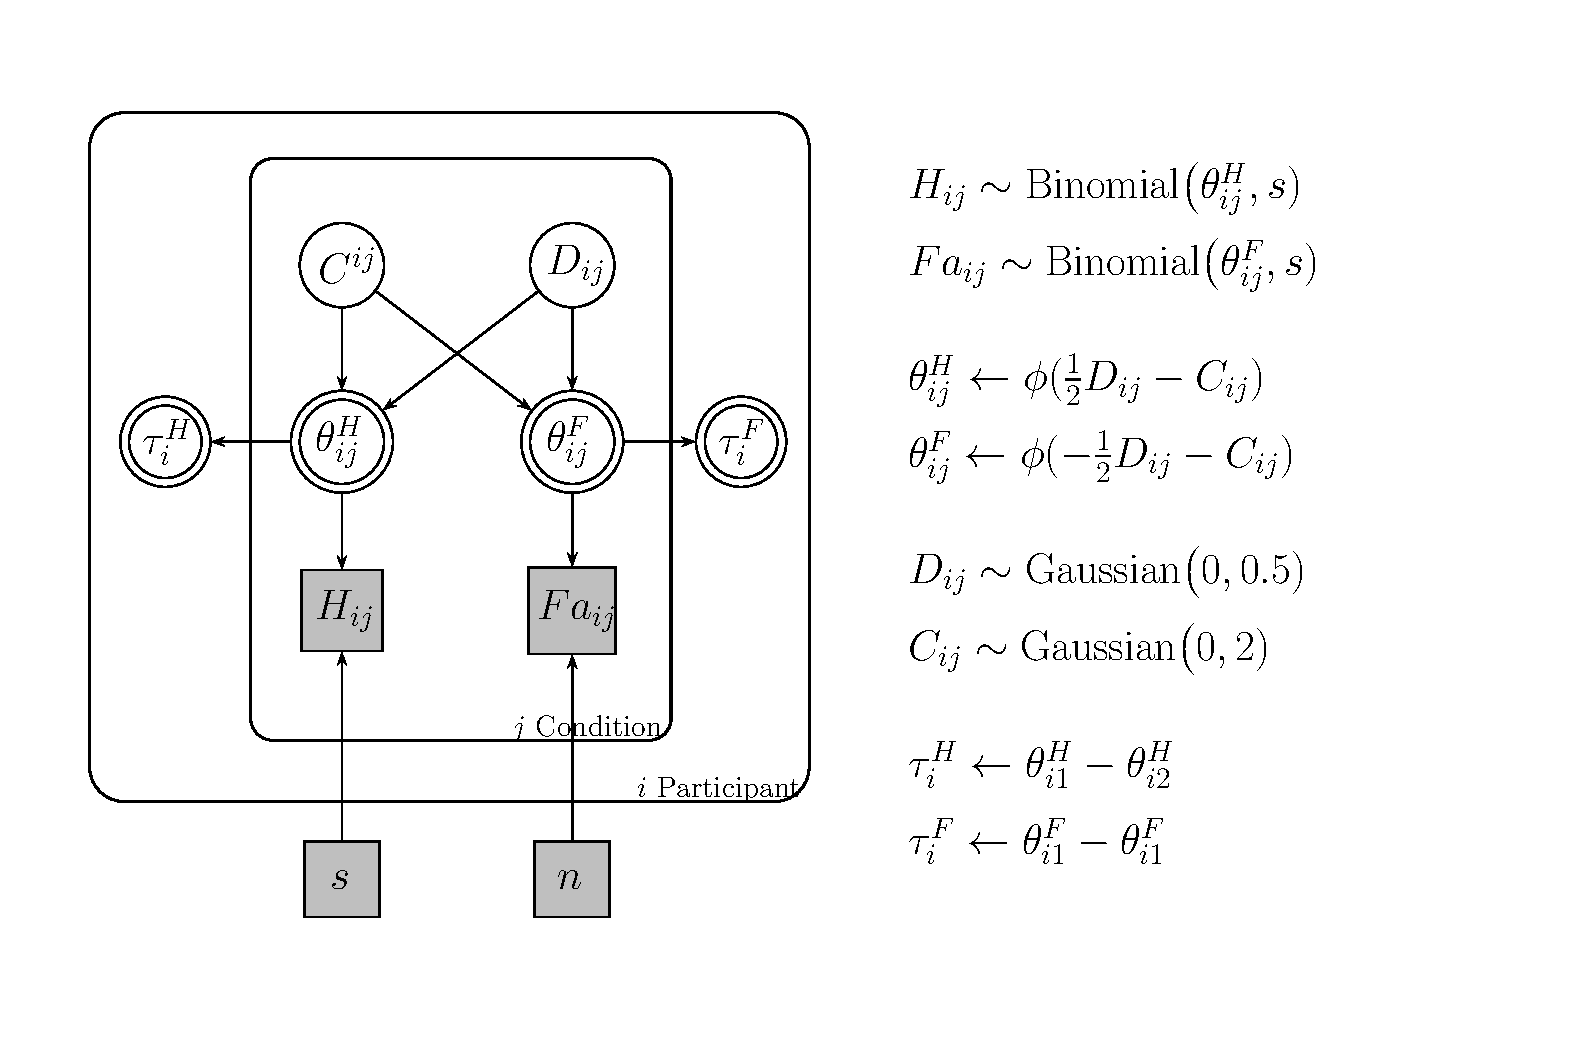
\includegraphics[width=0.80\textwidth]{Figures/Model_Tau_Diff_Tetas}
%\decoRule
\caption[Diferencias en Tasas (Comprobando diferencias entre condiciones)]{Comparación intrasujeto de}
\label{fig:Mod_Tau}
\end{figure}




\section{Diferencias en la asignación de Puntajes de Confianza}

\subsection{Análisis 1: }

\begin{table}
\caption[Prueba T]{Diferencias en los puntajes de confianza asignados a cada tipo de estímulo (Experimento 1 y 2)}
\label{Tabla_t-HitsyFA}
\centering
\begin{tabular}{l l |  c c c c}
\toprule
%\tabhead{Groups} & \tabhead{Treatment X} & \tabhead{Treatment Y} \\
\textbf{T-test} & \textbf{} & \textbf{$\mu$ A} & \textbf{$\mu$ B} & \textbf{T} & \textbf{P value}\\
\midrule
Exp 1 & Signal & 5.445 & 5.212 & -1.7778, & 0.0418 \\
Exp 1 & Noise & 1.542 & 1.883 & -1.7208 & 0.0472 \\
Exp 2 & Signal & 5.183 & 4.342  & -3.6752, & 0.0004 \\
Exp 2 & Noise & 2.386 & 2.752 & -1.809 & 0.0391 \\
\bottomrule
\end{tabular}
\end{table}



\section{Réplica de controles reportados en la literatura}



